% This is "sig-alternate.tex" V2.1 April 2013
% This file should be compiled with V2.5 of "sig-alternate.cls" May 2012
%
% This example file demonstrates the use of the 'sig-alternate.cls'
% V2.5 LaTeX2e document class file. It is for those submitting
% articles to ACM Conference Proceedings WHO DO NOT WISH TO
% STRICTLY ADHERE TO THE SIGS (PUBS-BOARD-ENDORSED) STYLE.
% The 'sig-alternate.cls' file will produce a similar-looking,
% albeit, 'tighter' paper resulting in, invariably, fewer pages.
%
% ----------------------------------------------------------------------------------------------------------------
% This .tex file (and associated .cls V2.5) produces:
%       1) The Permission Statement
%       2) The Conference (location) Info information
%       3) The Copyright Line with ACM data
%       4) NO page numbers
%
% as against the acm_proc_article-sp.cls file which
% DOES NOT produce 1) thru' 3) above.
%
% Using 'sig-alternate.cls' you have control, however, from within
% the source .tex file, over both the CopyrightYear
% (defaulted to 200X) and the ACM Copyright Data
% (defaulted to X-XXXXX-XX-X/XX/XX).
% e.g.
% \CopyrightYear{2007} will cause 2007 to appear in the copyright line.
% \crdata{0-12345-67-8/90/12} will cause 0-12345-67-8/90/12 to appear in the copyright line.
%
% ---------------------------------------------------------------------------------------------------------------
% This .tex source is an example which *does* use
% the .bib file (from which the .bbl file % is produced).
% REMEMBER HOWEVER: After having produced the .bbl file,
% and prior to final submission, you *NEED* to 'insert'
% your .bbl file into your source .tex file so as to provide
% ONE 'self-contained' source file.
%
% ================= IF YOU HAVE QUESTIONS =======================
% Questions regarding the SIGS styles, SIGS policies and
% procedures, Conferences etc. should be sent to
% Adrienne Griscti (griscti@acm.org)
%
% Technical questions _only_ to
% Gerald Murray (murray@hq.acm.org)
% ===============================================================
%
% For tracking purposes - this is V2.0 - May 2012

\documentclass{sig-alternate-05-2015}
\usepackage{epstopdf}
\usepackage[nomain, acronym, toc]{glossaries}
\usepackage{pgfplots}

\definecolor{rosso}{RGB}{220,57,18}
\definecolor{giallo}{RGB}{255,153,0}
\definecolor{blu}{RGB}{102,140,217}
\definecolor{verde}{RGB}{16,150,24}
\definecolor{viola}{RGB}{153,0,153}

\makeatletter

\tikzstyle{chart}=[
    legend label/.style={font={\scriptsize},anchor=west,align=left},
    legend box/.style={rectangle, draw, minimum size=5pt},
    axis/.style={black,semithick,->},
    axis label/.style={anchor=east,font={\tiny}},
]

\tikzstyle{bar chart}=[
    chart,
    bar width/.code={
        \pgfmathparse{##1/2}
        \global\let\bar@w\pgfmathresult
    },
    bar/.style={very thick, draw=white},
    bar label/.style={font={\bf\small},anchor=north},
    bar value/.style={font={\footnotesize}},
    bar width=.75,
]

\tikzstyle{pie chart}=[
    chart,
    slice/.style={line cap=round, line join=round, very thick,draw=white},
    pie title/.style={font={\bf}},
    slice type/.style 2 args={
        ##1/.style={fill=##2},
        values of ##1/.style={}
    }
]

\pgfdeclarelayer{background}
\pgfdeclarelayer{foreground}
\pgfsetlayers{background,main,foreground}


\newcommand{\pie}[3][]{
    \begin{scope}[#1]
    \pgfmathsetmacro{\curA}{90}
    \pgfmathsetmacro{\r}{1}
    \def\c{(0,0)}
    \node[pie title] at (90:1.3) {#2};
    \foreach \v/\s in{#3}{
        \pgfmathsetmacro{\deltaA}{\v/100*360}
        \pgfmathsetmacro{\nextA}{\curA + \deltaA}
        \pgfmathsetmacro{\midA}{(\curA+\nextA)/2}

        \path[slice,\s] \c
            -- +(\curA:\r)
            arc (\curA:\nextA:\r)
            -- cycle;
        \pgfmathsetmacro{\d}{max((\deltaA * -(.5/50) + 1) , .5)}

        \begin{pgfonlayer}{foreground}
        \path \c -- node[pos=\d,pie values,values of \s]{$\v\%$} +(\midA:\r);
        \end{pgfonlayer}

        \global\let\curA\nextA
    }
    \end{scope}
}

\newcommand{\legend}[2][]{
    \begin{scope}[#1]
    \path
        \foreach \n/\s in {#2}
            {
                  ++(0,-10pt) node[\s,legend box] {} +(5pt,0) node[legend label] {\n}
            }
    ;
    \end{scope}
}

% Acronym Definition

\newacronym{IST}{IST}{Instituto Superior T\'ecnico}
\newacronym{IoT}{IoT}{Internet of Things}
\newacronym{MQTT}{MQTT}{Message Queue Telemetry Transport}
\newacronym{MQTT-SN}{MQTT-SN}{Message Queue Telemetry Transport for Sensor Networks}
\newacronym{CoAP}{CoAP}{Constrained Application Protocol}
\newacronym{HTTP}{HTTP}{Hypertext Transfer Protocol}
\newacronym{TLS}{TLS}{Transport Layer Security}
\newacronym{DTLS}{DTLS}{Datagram Transport Layer Security}
\newacronym{WWW}{WWW}{World Wide Web}
\newacronym{MTU}{MTU}{Maximum Transmission Unit}
\newacronym{TCP}{TCP}{Transmission Control Protocol}
\newacronym{REST}{REST}{REpresentational State Transfer}
\newacronym{UDP}{UDP}{User Datagram Protocol}
\newacronym{URIs}{URIs}{Universal Resource Identifiers}
\newacronym{M2M}{M2M}{Machine to Machine}
\newacronym{QoS}{QoS}{Quality of Service}
\newacronym{WLAN}{WLAN}{Wireless Local Area Networks}
\newacronym{WPAN}{WPAN}{Wireless Private Area Networks}
\newacronym{LR-WPAN}{LR-WPAN}{Low-Rate Wireless Private Area Networks}
\newacronym{MAC}{MAC}{Medium Access Control}
\newacronym{FFD}{FFD}{Full Function Device}
\newacronym{RFD}{RFD}{Reduced Function Device}
\newacronym{IETF}{IETF}{Internet Engineering Task Force}
\newacronym{DoS}{DoS}{Denial of Service}
\newacronym{DODAG}{DODAG}{Destination Oriented Directed Acyclic Graph}
\newacronym{DIO}{DIO}{DODAG Information Objects}
\newacronym{DAO}{DAO}{Destination Advertisement Objects}
\newacronym{DIS}{DIS}{DODAG Information Solicitation}
\newacronym{RFID}{RFID}{Radio Frequency Identification}
\newacronym{ACL}{ACL}{Access Control List}
\newacronym{6LoWPAN}{6LoWPAN}{IPv6 over Low power Wireless Personal Area Networks}
\newacronym{RPL}{RPL}{Routing Protocol for Low-Power and Lossy Networks}
\newacronym{CA}{CA}{Certificate Authority}
\newacronym{CSDS}{CSDS}{\gls{CoAP} Service Discovery Server}
\newacronym{RDC}{RDC}{Radio Duty Cycling}

\begin{document}

% Copyright
\setcopyright{acmcopyright}
%\setcopyright{acmlicensed}
%\setcopyright{rightsretained}
%\setcopyright{usgov}
%\setcopyright{usgovmixed}
%\setcopyright{cagov}
%\setcopyright{cagovmixed}


% DOI
\doi{10.475/123_4}

% ISBN
\isbn{123-4567-24-567/08/06}

%Conference
\conferenceinfo{PLDI '13}{June 16--19, 2013, Seattle, WA, USA}

\acmPrice{\$15.00}

%
% --- Author Metadata here ---
\conferenceinfo{ACSAC}{'16 Los Angeles, California USA}
%\CopyrightYear{2007} % Allows default copyright year (20XX) to be over-ridden - IF NEED BE.
%\crdata{0-12345-67-8/90/01}  % Allows default copyright data (0-89791-88-6/97/05) to be over-ridden - IF NEED BE.
% --- End of Author Metadata ---

\title{Securing Smart Places: A Power-Aware Infrastructure}
%
% You need the command \numberofauthors to handle the 'placement
% and alignment' of the authors beneath the title.
%
% For aesthetic reasons, we recommend 'three authors at a time'
% i.e. three 'name/affiliation blocks' be placed beneath the title.
%
% NOTE: You are NOT restricted in how many 'rows' of
% "name/affiliations" may appear. We just ask that you restrict
% the number of 'columns' to three.
%
% Because of the available 'opening page real-estate'
% we ask you to refrain from putting more than six authors
% (two rows with three columns) beneath the article title.
% More than six makes the first-page appear very cluttered indeed.
%
% Use the \alignauthor commands to handle the names
% and affiliations for an 'aesthetic maximum' of six authors.
% Add names, affiliations, addresses for
% the seventh etc. author(s) as the argument for the
% \additionalauthors command.
% These 'additional authors' will be output/set for you
% without further effort on your part as the last section in
% the body of your article BEFORE References or any Appendices.

\numberofauthors{2} %  in this sample file, there are a *total*
% of EIGHT authors. SIX appear on the 'first-page' (for formatting
% reasons) and the remaining two appear in the \additionalauthors section.
%
\author{
% You can go ahead and credit any number of authors here,
% e.g. one 'row of three' or two rows (consisting of one row of three
% and a second row of one, two or three).
%
% The command \alignauthor (no curly braces needed) should
% precede each author name, affiliation/snail-mail address and
% e-mail address. Additionally, tag each line of
% affiliation/address with \affaddr, and tag the
% e-mail address with \email.
%
% 1st. author
\alignauthor
Tiago Diogo\\
       \affaddr{Instituto Superior Técnico}\\
       \affaddr{Av. Rovisco Pais, 1}\\
       \affaddr{1049-001 Lisboa, Portugal}\\
       \email{tiago.diogo@tecnico.ulisboa.pt}
% 2nd. author
\alignauthor
Miguel Pardal\\
       \affaddr{Inesc ID}\\
       \affaddr{Rua Alves Redol, 9}\\
       \affaddr{1000-029 Lisboa, Portugal}\\
       \email{miguel.pardal@tecnico.ulisboa.pt}
}
% There's nothing stopping you putting the seventh, eighth, etc.
% author on the opening page (as the 'third row') but we ask,
% for aesthetic reasons that you place these 'additional authors'
% in the \additional authors block, viz.

% Just remember to make sure that the TOTAL number of authors
% is the number that will appear on the first page PLUS the
% number that will appear in the \additionalauthors section.

\maketitle
\begin{abstract}
The \gls{IoT} and its vision of connecting every device to one another presents an opportunity to create large information sharing networks. However, intruders can take advantage of the \gls{IoT} devices constrained nature to disrupt these networks and launch a wide range of attacks on its nodes.
In our work we address this issue from a power-aware perspective, trying to find the best relation between security and power consumption. To achieve this objective we do a thoroughly analysis of the existing protocols, attacks and mitigation strategies, combining that information into our proposed smart places network management system.
Furthermore, energy consumption profiling was performed to endow future users with the knowledge of what kind of physical resources to deploy, based on the desired network security characteristics.
\end{abstract}


%
% The code below should be generated by the tool at
% http://dl.acm.org/ccs.cfm
% Please copy and paste the code instead of the example below. 
%
\begin{CCSXML}
<ccs2012>
<concept>
<concept_id>10010520.10010553.10003238</concept_id>
<concept_desc>Computer systems organization~Sensor networks</concept_desc>
<concept_significance>500</concept_significance>
</concept>
<concept>
<concept_id>10002978.10003014.10003017</concept_id>
<concept_desc>Security and privacy~Mobile and wireless security</concept_desc>
<concept_significance>300</concept_significance>
</concept>
</ccs2012>  
\end{CCSXML}

\ccsdesc[500]{Computer systems organization~Sensor networks}
\ccsdesc[300]{Security and privacy~Mobile and wireless security}


%
% End generated code
%

%
%  Use this command to print the description
%
\printccsdesc

% We no longer use \terms command
%\terms{Theory}

\keywords{Internet of Things; Power-Aware Security; Secure Bootstrapping; CoAP; 6LoWPAN; RPL; IEEE 802.15.4}

\section{Introduction}
The Internet of Things can be seen as a web of interconnected devices that go from everyday wearable objects into fully deployed sensor networks. Despite the huge variety and characteristics of these devices, one thing that they all have in common is the constrained nature that they are built upon. In order to enable the massive deployment to be expected in the near future, \gls{IoT} devices must be accessible and affordable, capable of operating under lossy wireless networks while being battery powered. This poses a challenge to current Internet protocols since the assumptions regarding the devices' capabilities and objectives do not hold true.\\ To allow the \gls{IoT} vision to come forward, several new protocols have been developed across the OSI layers, each addressing and tackling the challenges involved in trying to keep the quality and assurances of stronger, more expensive protocols, on constrained systems. After being thoroughly analysed, these protocols have been selected and grouped in a power-efficient stack, establishing a base line for power consumption.
Additionally, major attention has been given to information security because for both corporations and individuals, the interconnection of the devices around us can provide information about our choices and whereabouts, therefore leaking corporate information or simply reducing our individual privacy \cite{Ukil2015}. Thus, the focus moved towards adding mechanism to ensure authentication, confidentiality and integrity of the transmitted information by securing the communication channel. This increased the infrastructure complexity and created the need for a management system capable of storing and flashing network credentials onto new nodes.
In order to understand the cost of adding these mechanisms, additional experiments have been performed so that the added power consumption can be measured, profiled and documented, enabling the finding of the best parameters and requirements for a desired level of security.

\section{Securing Smart Places}

\subsection{Protocol Analysis and Selection}
\paragraph{}
There are many alternatives and some proposed standards when it comes to choosing a protocol stack for \gls{IoT} communications. The decision must be based on the particularities of the devices to be used and the objective of the application itself, however a thorough analysis of the existing solutions is a proper way to unveil the strong and weak points of each protocol providing a good basis for an informed decision. A recent survey (January 2015) \cite{Al-Fuqaha2015} of \gls{IoT} enabling technologies, protocols and applications was the starting point for the analysis to follow. The presentation of the available protocols and solutions will follow a bottom-up approach, starting from the data link and physical layer all the way up until the application layer. In particular, the session layer will be left to the end since securing the channel is an optional feature and will be addressed after the application level protocols are properly examined.

\subsubsection{Data Link and Physical Layer}

\paragraph{}
The first requirement for the physical layer of the \gls{IoT} is the use of wireless radios. These should aim for simplicity, low-power and low-cost communications. While wireless communication is widespread and can be found from homes to airports, the type of radio commonly used, known as Wi-Fi, uses a high amount of power causing concerns for battery life. In the next paragraphs, an overview of Wi-Fi (IEEE 802.11) is given with the objective of comparing it with the IEEE 802.15.4, a protocol that aims to address these issues.

\paragraph{\textbf{IEEE 802.11}}
\paragraph{}
IEEE 802.11 \cite{IEEE2012} is a set of standards for \gls{WLAN} communications. They are the basis for the so called Wi-Fi. IEEE 802.11 is concerned with high speed, long ranges, message forwarding and high data throughput. These concerns directly clash with the \gls{IoT} objectives and account for the added power consumption of this protocol.

\paragraph{\textbf{IEEE 802.15.4}}
\paragraph{}
IEEE 802.15.4 \cite{IEEEComputerSociety2011} on the other hand was created for \gls{LR-WPAN} and its specifications focus on low power consumption, low data rate, low cost and high message throughput make it a strong candidate for \gls{IoT} applications.
	The IEEE 802.15.4 standard supports two types of network nodes, the \gls{FFD} that acts as coordinator or normal node, and the \gls{RFD} that is very simple, with very constrained resources and can only communicate with coordinators. The coordinators are responsible for controlling and maintaining the network. \gls{FFD} are capable of storing a routing table in their memory and can implement a full \gls{MAC}.
	IEEE 802.15.4 supports star, peer-to-peer (mesh) and cluster-tree topologies.
	Regarding performance, it would be unfair to directly compare the two, since IEEE 802.11 transmission power and receiver sensitivity are much greater than 802.15.4. Even if we limit both to a low power level, IEEE 802.11 still outperforms IEEE 802.15.4 in terms of packet delivery ratio, throughput, latency, jitter and average energy consumption. However this comes at the cost of a far lower transmission range \cite{Transmission2011}.
	We can conclude that for typical \gls{LR-WPAN} network requirements, IEEE 802.15.4 is better designed to address the constrained environment issues, while IEEE 802.11 would still be a suitable option if a short transmission range is not a problem.

\subsubsection{Network Layer}
\label{sec:network_layer}

\paragraph{\textbf{6LoWPAN}}
\paragraph{}
	The \gls{IoT} vision and its massive deployment can only be achieved through the use of IPv6. However, physical layers more suitable for communication over constrained networks pose some limitations to the use of the IPv6 messages. For example, the limited packet size in IEEE 802.15.4 based networks. To tackle these issues, the \gls{IETF} \gls{6LoWPAN} \cite{Shelby2012} working group developed a standard based on header compression to reduce the transmission overhead, fragmentation to meet the IPv6 \gls{MTU} requirements and forwarding to link-layer to support multi-hop delivery \cite{Hui2008}.
	\gls{6LoWPAN} is able to remove a major share of IPv6 overheads, being able to compress its headers to two bytes, therefore allowing small IPv6 datagrams to be sent over IEEE 802.15.4 networks. 
	
\paragraph{\textbf{RPL}}
\paragraph{}
With the use of 6LoWPAN, upper layer routing protocols can now use the IPv6 addressing scheme. Given the possible frequent topology changes associated with the radio-link instability, successful  solutions must take these requirements into account on their specification. \gls{RPL} \cite{Winter2012} can support a wide variety of link-layers and is prepared for devices with very limited resources. It is able to build up network routes, distribute routing knowledge among nodes and adapt the topology in a very efficient way. More in depth, \gls{RPL} creates a \gls{DODAG} between the 6LoWPAN network nodes (Figure \ref{fig:rpl_dodag}) that supports unidirectional traffic towards the \gls{DODAG} root and bidirectional traffic between devices. Each node has a rank that indicates its position relative to other nodes and with respect to the root. This rank is used to create optimized network paths. In order to allow packets to propagate downwards in the topology, either source routing or stateful routing tables are used (More Information on this two types of routing are given in sections \ref{sec:source_routing} and \ref{sec:tables_routing}). For both modes, the \gls{DODAG} root always maintains a complete list of the network nodes. \gls{RPL} provides a set of control messages in order to exchange routing graph information. \gls{DIO} are used to advertise information needed to build the \gls{DODAG}. \gls{DAO}  are used to advertise information so that downwards traffic can go through the nodes towards the leafs. Nodes may also resort to \gls{DIS} messages to request graph information from neighbour nodes. Finally, RPL has a built in topology repair mechanism that acts in the case of a routing topology failure, link failure or node failure. In case the topology needs to be rebuilt, a link layer metric is used to calculate the new route. The new path is considered fit for work if the link layer acknowledgements are received on it.

\begin{figure}[h!]
  \centering
  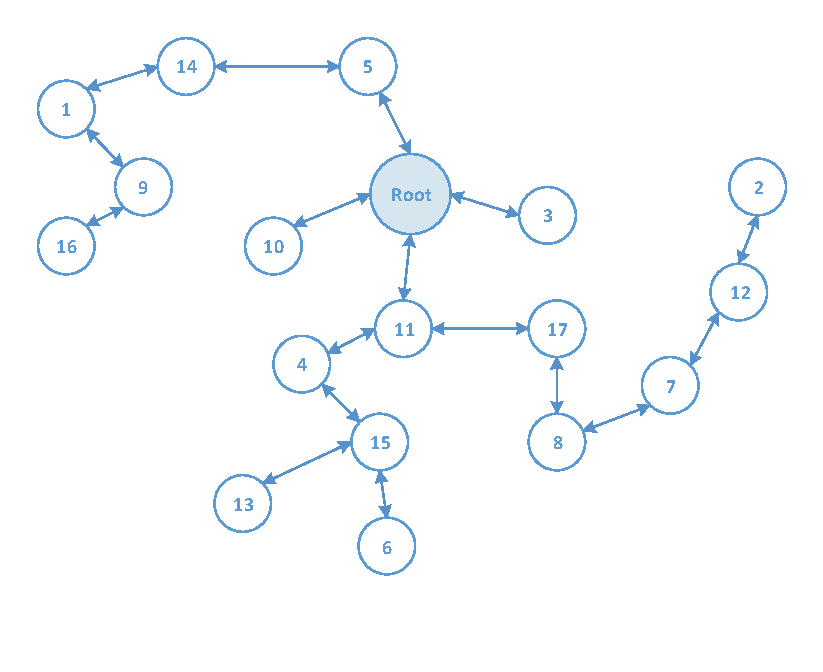
\includegraphics[width=1.0\linewidth]{figures/RPL_DODAG.pdf}
  \caption{A Sample RPL DODAG.}
  \label{fig:rpl_dodag}
\end{figure}

\subsubsection{Application Layer}

\paragraph{\textbf{\gls{HTTP}}}
\paragraph{}
	\gls{HTTP} is an application level protocol that uses a request-response model and is the foundation of data communication on the \gls{WWW} It is primarily designed to run over \gls{TCP} which is a problem in lossy and constrained environments due to the delivery assurances and congestion control algorithms it employs. Besides, {HTTP} is verbose, text-based, and not suited for compact message exchanges. Moreover, the header size required for a message exchange can leave too few payload space in constrained networks like the IEEE 802.15.4-based networks where the \gls{MTU} size of the protocol is 127 bytes. These protocol specifications would not raise any issues in standard \gls{WWW} communications, but when it comes to constrained environments it is clear that the protocol is not adequate to the necessities of \gls{IoT} devices and networks.

\paragraph{\textbf{\gls{CoAP}}}
\paragraph{}
	\gls{CoAP} \cite{Shelby2014} is a document transfer protocol based on \gls{REST} on top of \gls{HTTP} functionalities. \gls{CoAP} objective is to enable tiny constrained devices to use RESTful interactions, where clients and servers expose and consume web services using \gls{URIs} together with  \gls{HTTP} Get, Post, Put and Delete methods. Unlike \gls{REST}, \gls{CoAP} runs over \gls{UDP} instead of \gls{TCP} which makes it suitable for full IP networking in small micro-controllers. Retries and reordering are implemented at the application stack using a messaging sub-layer that detects duplicated messages and provides reliable communication using different types of messages. Confirmable messages must be acknowledged by the receiver, nonconfirmable follow the fire-and-forget model. Despite being a lightweight protocol, \gls{CoAP} still provides important features:
	
\begin{itemize}
	\item Resource Observation - \gls{CoAP} can extend the \gls{HTTP} request model with the ability to observe a resource therefore monitoring resources of interest using a publish/subscribe mechanism;\\
	\item Resource Discovery - \gls{CoAP} servers provide a list of resources using well-known {URIs} that allow clients to discover what resources are provided and their types;\\
	\item Interoperability - since \gls{CoAP} is based on the \gls{REST} architecture, a simple proxy enables \gls{CoAP} to easily interoperate with \gls{HTTP}.
\end{itemize}

\paragraph{}
A study that compared \gls{CoAP} and \gls{HTTP} using mobile networks concluded that there is no scenario where \gls{CoAP} would consume more resources than \gls{HTTP} \cite{Savolainen2014}.

\begin{table}[h]
	\centering
	\begin{center} \caption{Protocol Stack Comparison Overview } \label{tab:stack}\end{center}
	\begin{tabular}{c|c|c}
		Layer & Web & IoT \\
		\hline
		Application & \gls{HTTP} & \gls{CoAP} \\
		Transport & \gls{TCP} & \gls{UDP} \\
		Network & IPv6 & 6LoWPAN \\
		Data-Link/Physical & 802.11 & 802.15.4
	\end{tabular}
\end{table}

\subsection{Attack Analysis, Detection and Mitigation}
\label{sec:attack_analysis}
\paragraph{}
Exploitation of existing solutions in the forms of malicious attacks can be found at all the studied OSI layers. They can go from a physical intruder replacing some node on a sensor field to the well-known \gls{DoS} at the application layer. However, given the characteristics of the devices and networks used in \gls{IoT} combined with the power consumption focus of this work, a specific kind of attacks performed at the network layer is of special interest and importance: battery depletion attacks, also known as, ``vampire'' attacks.

\paragraph{}
Battery depletion attacks aim at draining the battery, ``life'', of the network devices, working over time to entirely disable a network, hence being called ``vampire'' attacks. These attacks do not focus on flooding the network with many packages, instead they drain the node's life by delaying the packets transmission. Many of the existing attacks are not protocol specific \cite{Vasserman2013}, while others target specific protocols and implementations \cite{Pongle2015}. The following attacks aim at giving an overview of the existing attack possibilities on different routing solutions as well as existing mitigation strategies. Additionally, a range of attacks that target the RPL routing protocol is also analysed. Since RPL is the selected protocol of our energy efficient stack, it is of special importance to consider and assure the mitigation of attacks that would drain the device's batteries by exploiting this light weight protocol's inner workings.   

\subsubsection{Stateless Protocols}
\label{sec:source_routing}
\paragraph{}
In systems that use this type of routing protocols, the source node specifies the entire route to the destination in the packet header. This means that intermediaries do not make decisions regarding the next hop, they only forward to the next node as specified in the original path therefore reducing the amount of computation performed and used energy. However, the source node must ensure that the route is valid at the time of sending and that the neighbour relations among the devices allow the specified forwarding path. Using this transmission scheme, a malicious device can specify paths through the network that are far from optimal, wasting energy at the intermediate nodes who follow the included malicious source route. The Carousel and Stretch Attacks are examples of these attacks.

\paragraph{\textbf{Carousel Attack}}
\paragraph{}
The objective of this attack is to send a packet along a route composed as a series of loops. This way, a single node may forward the malicious packet several times increasing the total energy consumption by a factor of the number of loops the attacker has introduced on the packet header path. It targets source routing protocols by exploiting the limited verification of the packet headers at the intermediary nodes. Figure \ref{fig:carousel_attack} shows an example where a vampire node created a path composed of circles around the network when it could have exited after the first hop through the D node.
 
\begin{figure}[h]
  \centering
  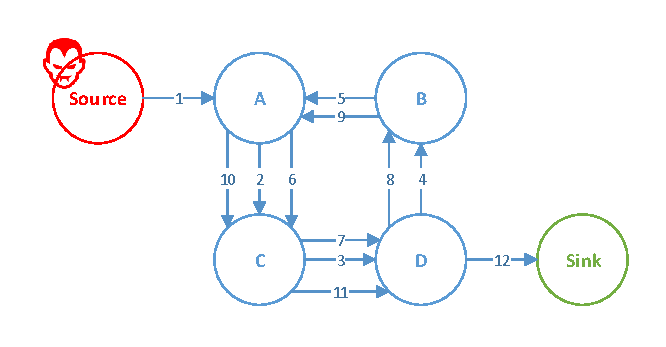
\includegraphics[width=0.9\linewidth]{figures/Carousel_Attack.pdf}
  \caption{Carousel Attack.}
  \label{fig:carousel_attack}
\end{figure}

Existing mitigation strategies rely on checking the source route for loops on intermediary nodes, either selecting an appropriate route for the packet or simply dropping it.

\paragraph{\textbf{Stretch Attack}}
\paragraph{}
The objective of this attack is to create a source route around the network, longer than the one that would be required to transverse the network from the source to the sink. The number of elements in the path would be greater than the optimal path, therefore increasing the total energy consumption by a factor of the number of additional hops. Its success rests on intermediary nodes not checking for better paths. Figure \ref{fig:stretch_attack} shows an example where a vampire node created a path that goes through a greater number of nodes than required to reach the sink.

\begin{figure}[h]
  \centering
  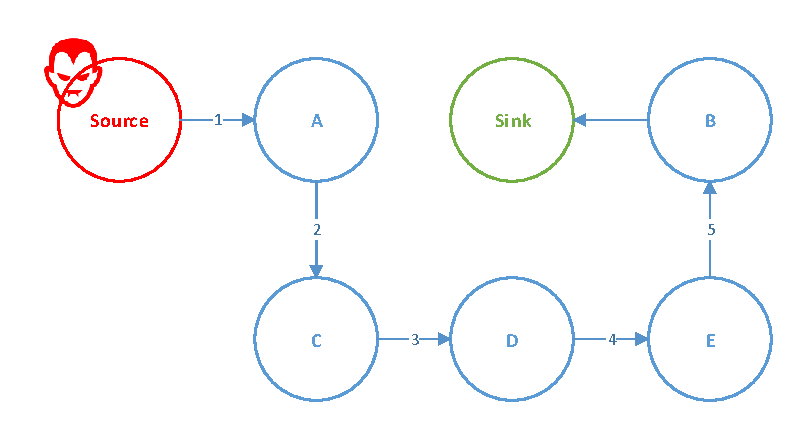
\includegraphics[width=0.8\linewidth]{figures/Stretch_Attack.pdf}
  \caption{Stretch Attack.}
  \label{fig:stretch_attack}
\end{figure}

A limited way of mitigating this attack would be to ensure that path routes have less than the total number of devices on the network. Vasserman and Hoper proposed a property called ``no-backtracking'' that assures the packet is always moving closer to the sink on every hop \cite{Vasserman2013}.
\pagebreak
\subsubsection{Stateful Protocols}
\label{sec:tables_routing}
\paragraph{}
In systems that use this type of routing protocols, network nodes are aware of the network topology and its state, being able to make local decisions on the node to whom they will forward the packet. The effect of the Vampires on this type of routing is limited since the route is built dynamically from many independent forwarding decisions. However, attackers can still cause damage by forcing packet forwarding through nodes that would not be on the optimal path, for example, by forwarding the packet back to the source. The Directional Antenna and Wormhole Attacks are examples of these attacks.

\paragraph{\textbf{Directional Antenna Attack}}
\paragraph{}
In this attack, the attacker takes the role of an intermediary and not the source of a packet. If the attacker has the resources to use a directional antenna, it can deposit a packet on arbitrary parts of the network while also forwarding the packet locally. This causes nodes that were not on the optimal path to also consume energy by forwarding a packet they would not normally receive, therefore increasing the total energy consumption by a factor of the directions the attacker can position the antenna and the distance between the receiver and the sink. Figure \ref{fig:directional_antenna_attack} shows an example where a ``vampire'' intermediary deposited a node on a distant location of the network, causing the packet to follow two different routes towards its destination

\begin{figure}[h]
  \centering
  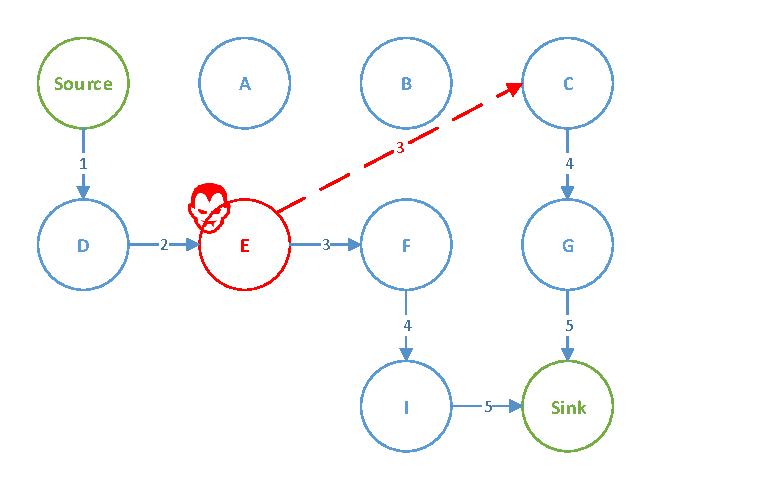
\includegraphics[width=0.8\linewidth]{figures/Directional_Antenna_Attack.pdf}
  \caption{Directional Antenna Attack.}
  \label{fig:directional_antenna_attack}
\end{figure}

A mitigation strategy could be to analyse the route paths of a given packet that reached the sink more than once. The last node identifier to appear duplicated before the path started to diverge would be one who then directed the packet to multiple regions, therefore revealing the attacker.

\paragraph{\textbf{Wormhole Attack}}
\paragraph{}
This attack can be seen as variation of the Directional Antenna Attack but with the collaboration of two or more attackers. Instead of simply forwarding the packets to arbitrary parts of the network, the attacker emulates a link between them and advertises to the network that recently formed connection. This disrupts the topology and has severe impact on routing paths since attackers can indicate that the link cost between them is very low, and therefore influence the forwarding decisions of neighbour nodes. By using these malicious routes, the energy consumption is increased because either this channel does not exist at all (packets are dropped and need to be resent), or the transmission cost between the attackers is greater than the normal message propagation through the network. Figure \ref{fig:wormhole_attack} shows an example where two vampires emulate a connection between them influencing the routing decisions of their neighbours. The hops numbered with prime numbers represent the path taken by a packet after the wormhole is constructed. Although the packet still reached the destination, the cost of the wormhole path is greater than the previous regular path.

\begin{figure}[h]
  \centering
  \includegraphics[width=0.85\linewidth]{figures/Wormhole_attack.pdf}
  \caption{Wormhole Attack.}
  \label{fig:wormhole_attack}
\end{figure} 

Wormhole attacks can be prevented using the Merkle tree authentication \cite{Khan2013}. This tree is organized from the leafs towards the root where every parent knows their children and asks them for authentication based on their ID and public key.
\pagebreak

\subsubsection{RPL Specific Attacks}
\paragraph{} 


\paragraph{\textbf{Selective Forwarding Attack}}
\paragraph{}
In a selective forwarding attack, a malicious node can launch a \gls{DoS} attack by selectively forwarding packets. Its main goal is to disrupt routing paths but can be used to filter any protocol. Since \gls{RPL} has built in topology repair mechanisms, a full packet filtering would trigger a healing phase and leave the malicious node out of the topology. For sustainability, an attacker could let the RPL control messages pass by and drop the remaining packets. Depending on the routing scheme being used (source routing or stateful tables) the source could first verify path availability or each node could dynamically decide to forward the packet through another path with similar quality. In any case, a good approach would be to report those failures to the underlying RPL system in order to trigger a preventive healing and improve the route quality.

\paragraph{\textbf{Hello Flooding Attack}}
\paragraph{}
The Hello in the name of this attack comes from the initial message a node sends when joining a network. By broadcasting this message with a strong signal power, an attacker can try to introduce himself as neighbour to many nodes of the network, or at least force a large portion of the network to spend energy starting the message exchange for node insertion. A simple solution for this attack would be to test the bi-directionality of the link. If no acknowledgement is received, the path is discarded. Another approach, if geographical locations of the nodes are known, would be to discard every hello message coming from a location beyond the transmission capabilities of ordinary nodes.

\subsubsection{Protocol Independent Attacks}
\paragraph{}
The last addressed category is not dependant on network topologies or protocol messages. It focuses on attacks that can be performed regardless of the used protocol and whose goal is to obtain information about a network device. With that information an attacker can, for example, try to include himself in the network as a legitimate device or spoof his identity to forward traffic towards him. The Clone and Sybil Attacks are examples of these attacks.

\paragraph{\textbf{Clone ID and Sybil Attack}}
\paragraph{}
As the name suggests, in a clone ID attack, the attacker steals the identity of a legitimate network node by copying the information of that node onto another node. This way the attacker can gain access to the traffic that was destined to the legitimate node, prevent packets to reach their intended destination and can even influence voting schemes. The Sybil attack is similar to the Clone ID, with the difference that the attacker uses several stolen identities on the same physical node. This way, large parts of a network can be taken over without the need to deploy several physical nodes. Figure \ref{fig:clone_attack} shows an example of a clone ID attack where the cloned attacker received the packet that was originally destined to the legitimate node.

\begin{figure}[h]
  \centering
  \includegraphics[width=0.85\linewidth]{figures/Clone_attack.pdf}
  \caption{Clone ID Attack.}
  \label{fig:clone_attack}
\end{figure} 

Proposed mitigation strategies for this type of attacks consist on keeping track of the number of instances of each identity. By using the node neighbours, either a centralized or distributed approach could be used to detect duplicate entries.

\subsection{Secure Bootstrapping}
\label{sec:secure_bootstrapping}
\paragraph{}
The term bootstrapping is applied to the process in which a new device is connected to an existing network. To achieve a secure bootstrapping, a unique identity and security parameters are associated with the device during this phase. There are several ways to carry out the initial setup, either via a physical interface or wirelessly. In the case of wireless bootstrapping, attention must be given to eavesdropping so that the secure credentials cannot be intercepted.\\
Since many of the studied attacks are to be performed by a malicious intruder capable of interacting with the network, if we could assure a secure bootstrapping, meaning that the new node would be authenticated before becoming an active member of the network, a large portion of those attacks could no longer be performed. The following bootstrapping techniques were summarized in \cite{Fischer2012} and aim at providing secure bootstrapping for \gls{IoT} devices.

\subsubsection{Token-Based}
\paragraph{}
In token-based distribution, device specific security credentials are generated and written to a token. That token can range from memory sticks or flash cards to \gls{RFID} tags or smartcards. Is has the advantage that this initial credential generation can be performed on a physically controlled environment and only later, on the commissioning phase, is the token plugged into the device. After the successful insertion of the security credentials, the token can be removed and collected back into the secure environment. This process can be considered of high security since the credentials are generated on a closed environment and are transmitted through a physical link. To further increase the security level, a password could be used to encrypt the credentials, however, that would require the device to have some kind of interface that would allow to input the password. In the case of a large number of devices, this approach would be unsuitable due to the management effort of manually deploying the tokens to the devices \cite{Fischer2012}.

\subsubsection{Identifier-Based Access Control List}
\paragraph{}
With an identifier based \gls{ACL}, new devices are allowed or denied access to the network based on their unique ID. A commonly used identifier is the MAC address. This has some major drawbacks in security since, firstly, it provides no assurances on the first time the device connects to the network. An attacker can easily intercept the first messages and get access to the device information. And secondly, after the bootstrapping phase, MAC addresses can be spoofed by an attacker, allowing him access to the network by bypassing the \gls{ACL} with the identifier of a legitimate node.

\subsubsection{One-Time-Passwords}
\paragraph{}
The use of one-time-passwords enhances the manual input of credentials on the device to be bootstrapped. The person responsible for the deployment of the new node should receive through a secure channel an one-time-password, that would then be used to authenticate the node, by authenticating its locally generated key material. This material can be either a certificate request to a \gls{CA} or a locally generated public/private key pair. The achieved security level is proportional to the security of the channel used to obtain the one time password, but assuming that channel is secure, so is this method. The drawback is that it forces devices to possess some kind of interface to insert the one time password.

\subsubsection{Manufacturer Installed Credentials}
\paragraph{}
So far, excluding the identifier based access control list, the intent of the studied techniques is to supply to the new device the security credentials needed to obtain access to the network, or at least provide an authentication method that allows fetching those credentials. In manufacturer installed credentials, those security credentials are deployed during the manufacturing process of the device vendor. Those credentials are typically a public/private key pair certificate bound to the identifier of the device. This certificate can be integrated into the initial loading of the firmware or stored in a separate integrated circuit designed for credential storing. In the second case, this method's security can be considered very high since those integrated circuits assure that the private key cannot be read from memory. This way, the new device comes shipped with the necessary security credentials not only for the bootstrapping phase but also for the normal operation phase since it does not need to fetch any additional credentials. The effort is on the root or management station that needs to import the vendor \gls{CA} certificates to assure the new device credentials are trustworthy. Also the production costs increase, implying an increased device cost.

\subsection{System Architecture}
A numbered display equation -- one set off by vertical space
from the text and centered horizontally -- is produced
by the \textbf{equation} environment. An unnumbered display
equation is produced by the \textbf{displaymath} environment.

Again, in either environment, you can use any of the symbols
and structures available in \LaTeX; this section will just
give a couple of examples of display equations in context.
First, consider the equation, shown as an inline equation above:
\begin{equation}\lim_{n\rightarrow \infty}x=0\end{equation}
Notice how it is formatted somewhat differently in
the \textbf{displaymath}
environment.  Now, we'll enter an unnumbered equation:
\begin{displaymath}\sum_{i=0}^{\infty} x + 1\end{displaymath}
and follow it with another numbered equation:
\begin{equation}\sum_{i=0}^{\infty}x_i=\int_{0}^{\pi+2} f\end{equation}
just to demonstrate \LaTeX's able handling of numbering.

\section{Evaluation}
In this section we measure and profile the resources required for the system operation. This ranges from the memory required for the nodes operative system and protocol stack, to power consumptions and battery replacement expectations. Each following subsection both presents the collected data and explains the process and technologies involved in obtaining it.

\subsection{Hardware Requirements}
In order to select hardware capable of supporting the stack of protocols used for communication it is necessary to measure the firmware size. For that task, the \texttt{msp430-size} tool was used. This tool analyses the firmware file and outputs the ammount of \texttt{text}, \texttt{data} and \texttt{bss}.\\
Text corresponds to code and constants, Data is for initialized variables and Bss is for uninitialized data (which is initialized with zero in the startup code).\\
The total amount of flash memory can me calculated from the sum of the text and data parameters.
The total amount of ram memory can be calculated from the sum of the data and bss parameters.


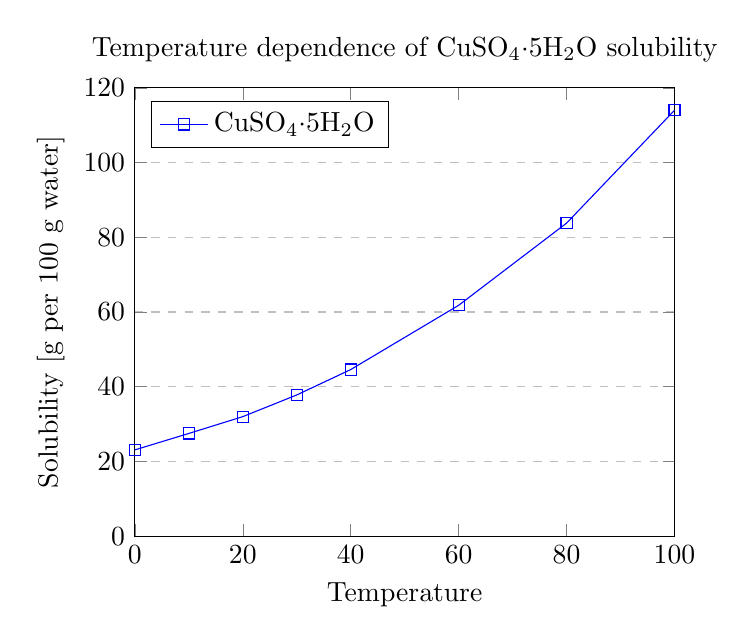
\begin{tikzpicture}
\begin{axis}[
    title={Temperature dependence of CuSO$_4\cdot$5H$_2$O solubility},
    xlabel={Temperature },
    ylabel={Solubility [g per 100 g water]},
    xmin=0, xmax=100,
    ymin=0, ymax=120,
    xtick={0,20,40,60,80,100},
    ytick={0,20,40,60,80,100,120},
    legend pos=north west,
    ymajorgrids=true,
    grid style=dashed,
]
 
\addplot[
    color=blue,
    mark=square,
    ]
    coordinates {
    (0,23.1)(10,27.5)(20,32)(30,37.8)(40,44.6)(60,61.8)(80,83.8)(100,114)
    };
    \legend{CuSO$_4\cdot$5H$_2$O}
 
\end{axis}
\end{tikzpicture}

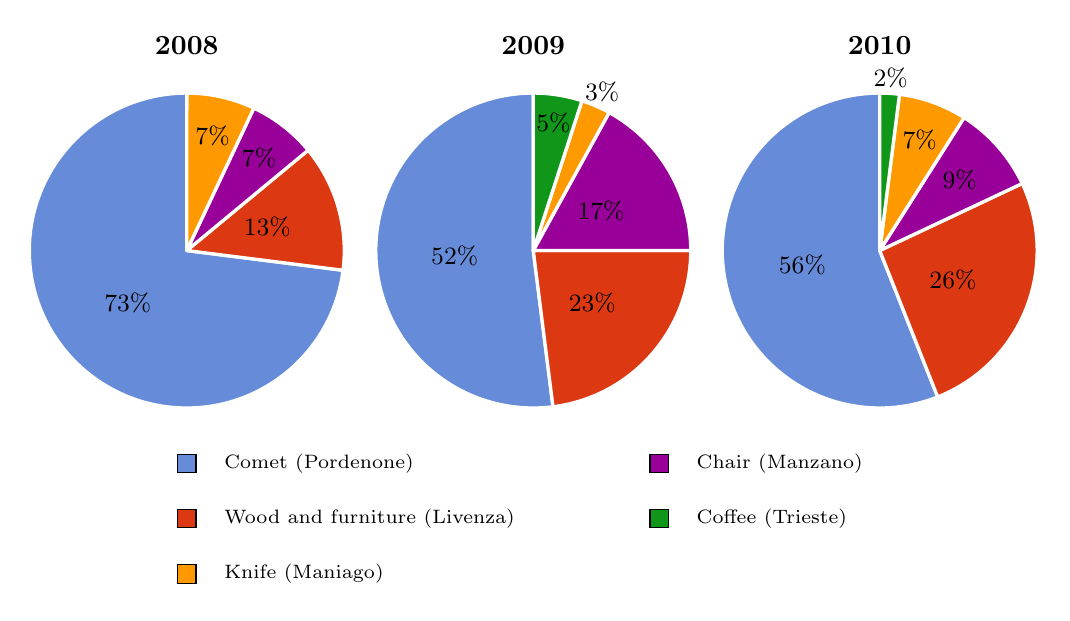
\begin{tikzpicture}
[
    pie chart,
    slice type={comet}{blu},
    slice type={legno}{rosso},
    slice type={coltello}{giallo},
    slice type={sedia}{viola},
    slice type={caffe}{verde},
    pie values/.style={font={\small}},
    scale=2
]

    \pie{2008}{73/comet,13/legno,7/sedia,7/coltello}
    \pie[xshift=2.2cm,values of coltello/.style={pos=1.1}]%
        {2009}{52/comet,23/legno,17/sedia,3/coltello,5/caffe}
    \pie[xshift=4.4cm,values of caffe/.style={pos=1.1}]%
        {2010}{56/comet,26/legno,9/sedia,7/coltello,2/caffe}

    \legend[shift={(0cm,-1cm)}]{{Comet (Pordenone)}/comet, {Wood and furniture (Livenza)}/legno, {Knife (Maniago)}/coltello}
    \legend[shift={(3cm,-1cm)}]{{Chair (Manzano)}/sedia, {Coffee (Trieste)}/caffe}

\end{tikzpicture}

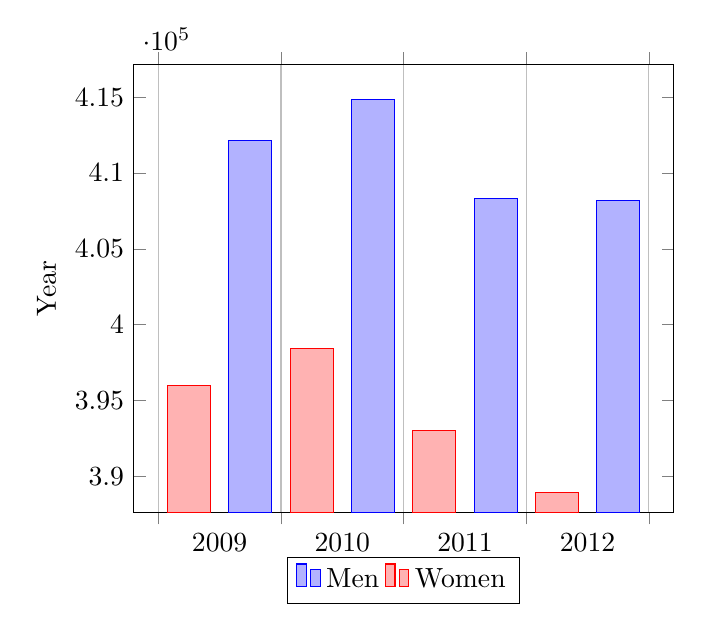
\begin{tikzpicture}
\begin{axis}[
	x tick label style={
		/pgf/number format/1000 sep=},
	ylabel=Year,
	enlargelimits=0.05,
	legend style={at={(0.5,-0.1)},
	anchor=north,legend columns=-1},
	ybar interval=0.7,
]
\addplot 
	coordinates {(2012,408184) (2011,408348)
		 (2010,414870) (2009,412156) (2008,415 838)};
\addplot 
	coordinates {(2012,388950) (2011,393007) 
		(2010,398449) (2009,395972) (2008,398866)};
\legend{Men,Women}
\end{axis}
\end{tikzpicture}


Citations to articles \cite{bowman:reasoning,
clark:pct, braams:babel, herlihy:methodology},
conference proceedings \cite{clark:pct} or
books \cite{salas:calculus, Lamport:LaTeX} listed
in the Bibliography section of your
article will occur throughout the text of your article.
You should use BibTeX to automatically produce this bibliography;
you simply need to insert one of several citation commands with
a key of the item cited in the proper location in
the \texttt{.tex} file \cite{Lamport:LaTeX}.
The key is a short reference you invent to uniquely
identify each work; in this sample document, the key is
the first author's surname and a
word from the title.  This identifying key is included
with each item in the \texttt{.bib} file for your article.

The details of the construction of the \texttt{.bib} file
are beyond the scope of this sample document, but more
information can be found in the \textit{Author's Guide},
and exhaustive details in the \textit{\LaTeX\ User's
Guide}\cite{Lamport:LaTeX}.

This article shows only the plainest form
of the citation command, using \texttt{{\char'134}cite}.
This is what is stipulated in the SIGS style specifications.
No other citation format is endorsed or supported.

\subsection{Hardware Requirements}
Because tables cannot be split across pages, the best
placement for them is typically the top of the page
nearest their initial cite.  To
ensure this proper ``floating'' placement of tables, use the
environment \textbf{table} to enclose the table's contents and
the table caption.  The contents of the table itself must go
in the \textbf{tabular} environment, to
be aligned properly in rows and columns, with the desired
horizontal and vertical rules.  Again, detailed instructions
on \textbf{tabular} material
is found in the \textit{\LaTeX\ User's Guide}.

Immediately following this sentence is the point at which
Table 1 is included in the input file; compare the
placement of the table here with the table in the printed
dvi output of this document.

\begin{table}
\centering
\caption{Frequency of Special Characters}
\begin{tabular}{|c|c|l|} \hline
Non-English or Math&Frequency&Comments\\ \hline
\O & 1 in 1,000& For Swedish names\\ \hline
$\pi$ & 1 in 5& Common in math\\ \hline
\$ & 4 in 5 & Used in business\\ \hline
$\Psi^2_1$ & 1 in 40,000& Unexplained usage\\
\hline\end{tabular}
\end{table}

To set a wider table, which takes up the whole width of
the page's live area, use the environment
\textbf{table*} to enclose the table's contents and
the table caption.  As with a single-column table, this wide
table will ``float" to a location deemed more desirable.
Immediately following this sentence is the point at which
Table 2 is included in the input file; again, it is
instructive to compare the placement of the
table here with the table in the printed dvi
output of this document.


\begin{table*}
\centering
\caption{Some Typical Commands}
\begin{tabular}{|c|c|l|} \hline
Command&A Number&Comments\\ \hline
\texttt{{\char'134}alignauthor} & 100& Author alignment\\ \hline
\texttt{{\char'134}numberofauthors}& 200& Author enumeration\\ \hline
\texttt{{\char'134}table}& 300 & For tables\\ \hline
\texttt{{\char'134}table*}& 400& For wider tables\\ \hline\end{tabular}
\end{table*}
% end the environment with {table*}, NOTE not {table}!

\subsection{Power Consumption}
Like tables, figures cannot be split across pages; the
best placement for them
is typically the top or the bottom of the page nearest
their initial cite.  To ensure this proper ``floating'' placement
of figures, use the environment
\textbf{figure} to enclose the figure and its caption.

This sample document contains examples of \textbf{.eps} files to be
displayable with \LaTeX.  If you work with pdf\LaTeX, use files in the
\textbf{.pdf} format.  Note that most modern \TeX\ system will convert
\textbf{.eps} to \textbf{.pdf} for you on the fly.  More details on
each of these is found in the \textit{Author's Guide}.

\begin{figure}
\centering
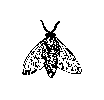
\includegraphics{fly}
\caption{A sample black and white graphic.}
\end{figure}

\begin{figure}
\centering
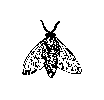
\includegraphics[height=1in, width=1in]{fly}
\caption{A sample black and white graphic
that has been resized with the \texttt{includegraphics} command.}
\end{figure}


As was the case with tables, you may want a figure
that spans two columns.  To do this, and still to
ensure proper ``floating'' placement of tables, use the environment
\textbf{figure*} to enclose the figure and its caption.
and don't forget to end the environment with
{figure*}, not {figure}!

\begin{figure*}
\centering
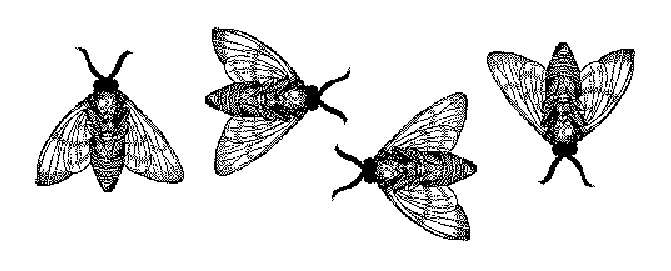
\includegraphics{flies}
\caption{A sample black and white graphic
that needs to span two columns of text.}
\end{figure*}


\begin{figure}
\centering
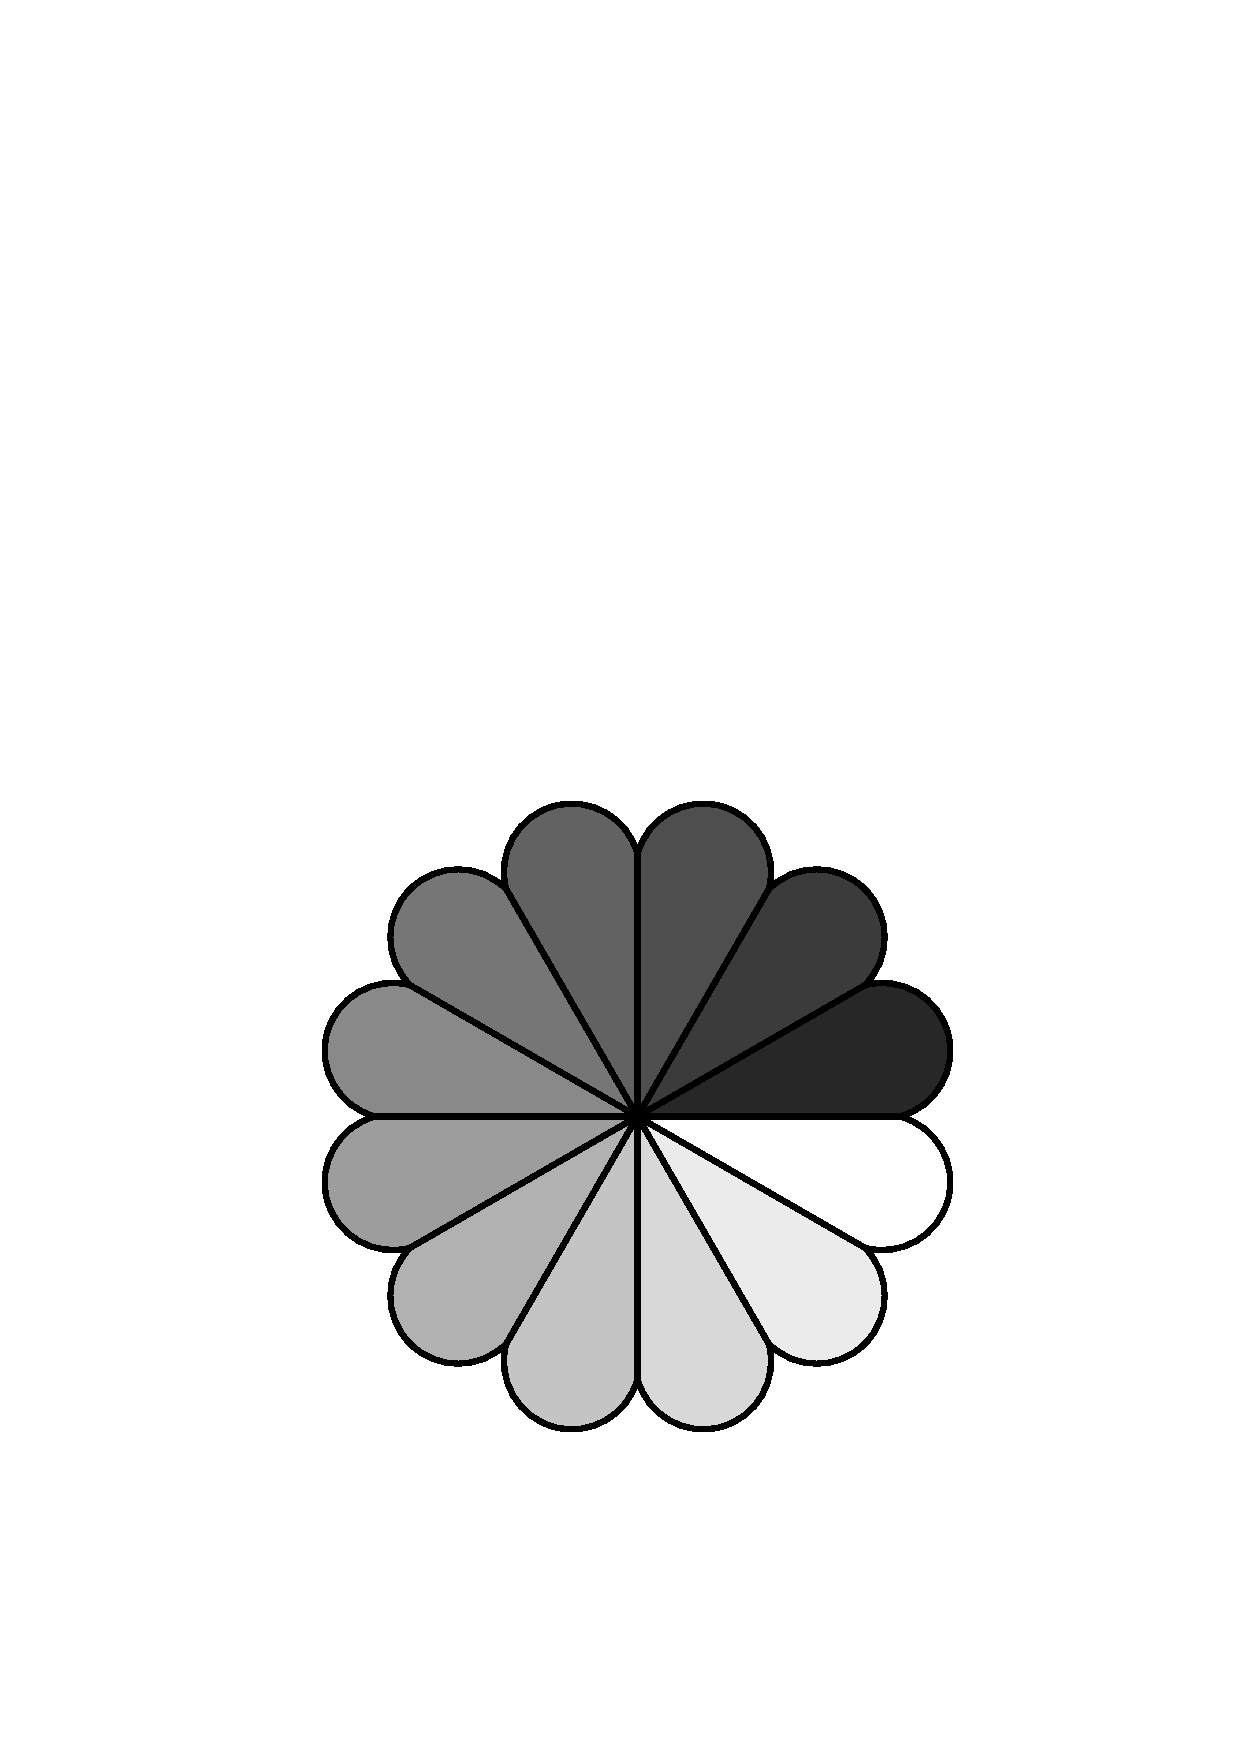
\includegraphics[height=1in, width=1in]{rosette}
\caption{A sample black and white graphic that has
been resized with the \texttt{includegraphics} command.}
\vskip -6pt
\end{figure}

\subsection{Theorem-like Constructs}
Other common constructs that may occur in your article are
the forms for logical constructs like theorems, axioms,
corollaries and proofs.  There are
two forms, one produced by the
command \texttt{{\char'134}newtheorem} and the
other by the command \texttt{{\char'134}newdef}; perhaps
the clearest and easiest way to distinguish them is
to compare the two in the output of this sample document:

This uses the \textbf{theorem} environment, created by
the\linebreak\texttt{{\char'134}newtheorem} command:
\newtheorem{theorem}{Theorem}
\begin{theorem}
Let $f$ be continuous on $[a,b]$.  If $G$ is
an antiderivative for $f$ on $[a,b]$, then
\begin{displaymath}\int^b_af(t)dt = G(b) - G(a).\end{displaymath}
\end{theorem}

The other uses the \textbf{definition} environment, created
by the \texttt{{\char'134}newdef} command:
\newdef{definition}{Definition}
\begin{definition}
If $z$ is irrational, then by $e^z$ we mean the
unique number which has
logarithm $z$: \begin{displaymath}{\log e^z = z}\end{displaymath}
\end{definition}

Two lists of constructs that use one of these
forms is given in the
\textit{Author's  Guidelines}.
 
There is one other similar construct environment, which is
already set up
for you; i.e. you must \textit{not} use
a \texttt{{\char'134}newdef} command to
create it: the \textbf{proof} environment.  Here
is a example of its use:
\begin{proof}
Suppose on the contrary there exists a real number $L$ such that
\begin{displaymath}
\lim_{x\rightarrow\infty} \frac{f(x)}{g(x)} = L.
\end{displaymath}
Then
\begin{displaymath}
l=\lim_{x\rightarrow c} f(x)
= \lim_{x\rightarrow c}
\left[ g{x} \cdot \frac{f(x)}{g(x)} \right ]
= \lim_{x\rightarrow c} g(x) \cdot \lim_{x\rightarrow c}
\frac{f(x)}{g(x)} = 0\cdot L = 0,
\end{displaymath}
which contradicts our assumption that $l\neq 0$.
\end{proof}

Complete rules about using these environments and using the
two different creation commands are in the
\textit{Author's Guide}; please consult it for more
detailed instructions.  If you need to use another construct,
not listed therein, which you want to have the same
formatting as the Theorem
or the Definition\cite{salas:calculus} shown above,
use the \texttt{{\char'134}newtheorem} or the
\texttt{{\char'134}newdef} command,
respectively, to create it.

\subsection*{A {\secit Caveat} for the \TeX\ Expert}
Because you have just been given permission to
use the \texttt{{\char'134}newdef} command to create a
new form, you might think you can
use \TeX's \texttt{{\char'134}def} to create a
new command: \textit{Please refrain from doing this!}
Remember that your \LaTeX\ source code is primarily intended
to create camera-ready copy, but may be converted
to other forms -- e.g. HTML. If you inadvertently omit
some or all of the \texttt{{\char'134}def}s recompilation will
be, to say the least, problematic.

\section{Conclusions}
This paragraph will end the body of this sample document.
Remember that you might still have Acknowledgments or
Appendices; brief samples of these
follow.  There is still the Bibliography to deal with; and
we will make a disclaimer about that here: with the exception
of the reference to the \LaTeX\ book, the citations in
this paper are to articles which have nothing to
do with the present subject and are used as
examples only.
%\end{document}  % This is where a 'short' article might terminate

%ACKNOWLEDGMENTS are optional
\section{Acknowledgments}
This section is optional; it is a location for you
to acknowledge grants, funding, editing assistance and
what have you.  In the present case, for example, the
authors would like to thank Gerald Murray of ACM for
his help in codifying this \textit{Author's Guide}
and the \textbf{.cls} and \textbf{.tex} files that it describes.

%
% The following two commands are all you need in the
% initial runs of your .tex file to
% produce the bibliography for the citations in your paper.
\bibliographystyle{abbrv}
\bibliography{sigproc}  % sigproc.bib is the name of the Bibliography in this case
% You must have a proper ".bib" file
%  and remember to run:
% latex bibtex latex latex
% to resolve all references
%
% ACM needs 'a single self-contained file'!
%
%APPENDICES are optional
%\balancecolumns
\appendix
%Appendix A
\section{Headings in Appendices}
The rules about hierarchical headings discussed above for
the body of the article are different in the appendices.
In the \textbf{appendix} environment, the command
\textbf{section} is used to
indicate the start of each Appendix, with alphabetic order
designation (i.e. the first is A, the second B, etc.) and
a title (if you include one).  So, if you need
hierarchical structure
\textit{within} an Appendix, start with \textbf{subsection} as the
highest level. Here is an outline of the body of this
document in Appendix-appropriate form:
\subsection{Introduction}
\subsection{The Body of the Paper}
\subsubsection{Type Changes and  Special Characters}
\subsubsection{Math Equations}
\paragraph{Inline (In-text) Equations}
\paragraph{Display Equations}
\subsubsection{Citations}
\subsubsection{Tables}
\subsubsection{Figures}
\subsubsection{Theorem-like Constructs}
\subsubsection*{A Caveat for the \TeX\ Expert}
\subsection{Conclusions}
\subsection{Acknowledgments}
\subsection{Additional Authors}
This section is inserted by \LaTeX; you do not insert it.
You just add the names and information in the
\texttt{{\char'134}additionalauthors} command at the start
of the document.
\subsection{References}
Generated by bibtex from your ~.bib file.  Run latex,
then bibtex, then latex twice (to resolve references)
to create the ~.bbl file.  Insert that ~.bbl file into
the .tex source file and comment out
the command \texttt{{\char'134}thebibliography}.
% This next section command marks the start of
% Appendix B, and does not continue the present hierarchy
\section{More Help for the Hardy}
The sig-alternate.cls file itself is chock-full of succinct
and helpful comments.  If you consider yourself a moderately
experienced to expert user of \LaTeX, you may find reading
it useful but please remember not to change it.
%\balancecolumns % GM June 2007
% That's all folks!
\end{document}

\newacronym{IST}{IST}{Instituto Superior T\'ecnico}
